\section{Force Main Design and Hygraulic Analysis}
\subsection{Layout and System Configuration}

The geometric configuration of the wastewater conveyance system establishes the basis for the hydraulic analysis of the force main and pump station. The system consists of a submersible lift station located within the Colebrooke Subdivision that conveys wastewater through a pressurized force main to an existing municipal gravity sewer manhole.

The alignment of the force main, including stationing, pipeline length, and connection points, was defined using Autodesk Civil 3D based on the subdivision survey and utility layout. The pipeline extends from the pump station at Sta.~0+00.00 to the receiving municipal manhole at Sta.~0+77.48, resulting in a total force main length of $77.48~\text{ft}$. The plan layout, shown in Figure~\ref{fig:force_main_plan_ch5}, identifies the pump station location, force main alignment, and downstream connection to the municipal sewer system.

\begin{figure}[H]
\centering
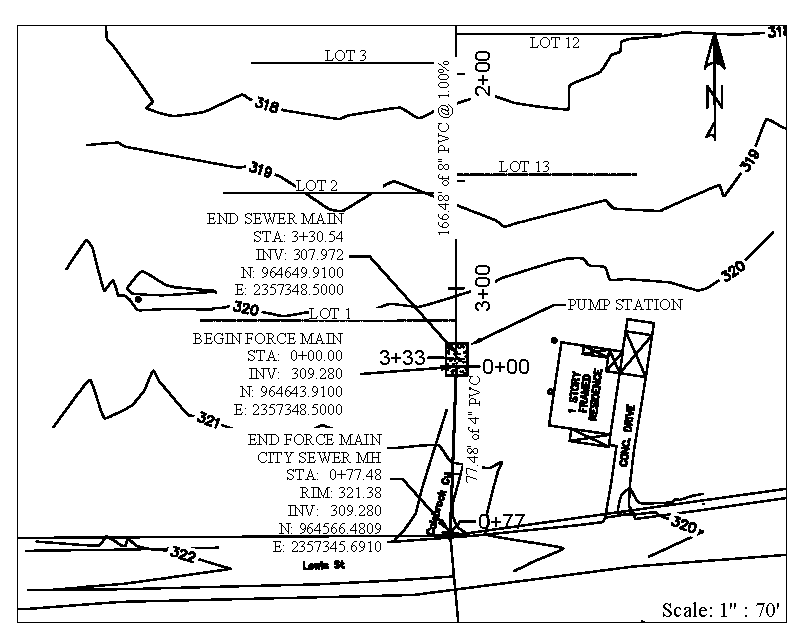
\includegraphics[width=\textwidth]{ForcemainLayoutPlan.pdf}
\caption{Final force main layout showing pump station location, pipeline alignment, and connection to the municipal sewer manhole.}
\label{fig:force_main_plan_ch5}
\end{figure}

The hydraulic profile of the system is defined by the wet well operating elevation of $299.00~\text{ft}$ and the discharge elevation of $309.28~\text{ft}$ at the receiving manhole. The profile, shown in Figure~\ref{fig:force_main_profile_ch5}, establishes the vertical relationship between the pump station and the municipal sewer system and defines the elevation difference governing the static head component of the hydraulic analysis.

\begin{figure}[H]
\centering
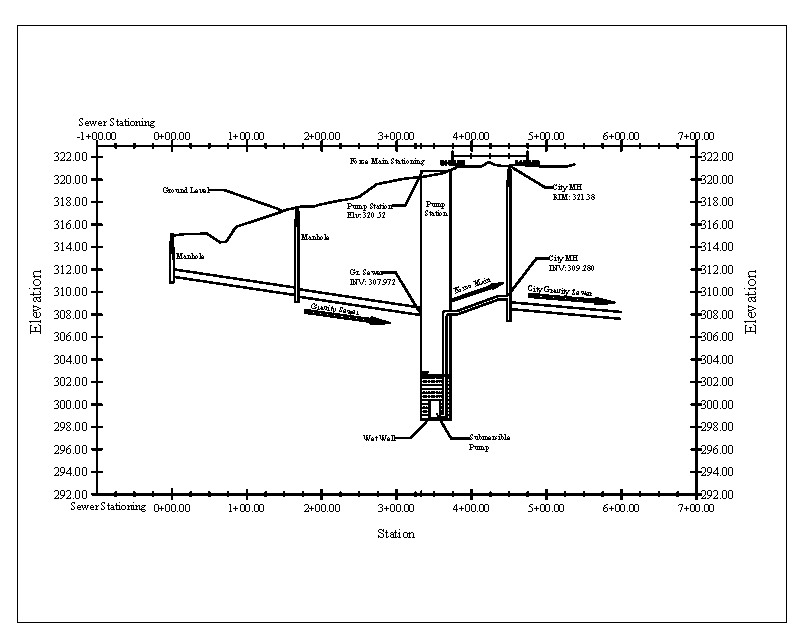
\includegraphics[width=\textwidth]{ForceMainLayoutProfile.pdf}
\caption{Hydraulic profile showing wet well elevation, force main alignment, and discharge elevation at the receiving municipal sewer manhole.}
\label{fig:force_main_profile_ch5}
\end{figure}

The plan and profile drawings provide the geometric inputs required for evaluating static head, friction losses, and minor losses in the force main. These parameters are used in the following sections to develop the total dynamic head and establish the system curve for pump selection.


\subsection{Design Parameters and Inputs}

The hydraulic design of the force main and pump station is based on the governing flow conditions, geometric configuration, and system parameters defined in Chapter~2. These inputs establish the basis for the evaluation of static head, friction losses, and minor losses used in the development of the total dynamic head.

The design flow for the system is taken as the peak wastewater inflow to the pump station, which is

\[
Q_{\text{peak}} = 12.46~\text{gpm}
\]

This flow represents the maximum anticipated inflow from the subdivision gravity sewer system and defines the minimum conveyance requirement for the pump station design.

In addition to the design flow, the hydraulic analysis requires geometric and system-specific parameters including the force main length, elevation data, pipe roughness coefficient, and minor loss coefficients. These parameters are summarized in Table~\ref{tab:design_inputs_ch5}.

\begin{table}[H]
\centering
\caption{Design Parameters for Hydraulic Analysis}
\label{tab:design_inputs_ch5}
\begin{tabular}{llll}
\toprule
\textbf{Parameter} & \textbf{Value} & \textbf{Unit} & \textbf{Description} \\
\midrule
Peak wastewater flow ($Q$) & 12.46 & gpm & Design inflow to pump station \\
Force main length ($L$) & 77.48 & ft & Distance from pump station to discharge \\
Discharge elevation ($z_d$) & 309.28 & ft & Receiving sewer manhole invert \\
Wet well elevation ($z_w$) & 299.00 & ft & Pump-off water surface elevation \\
Hazen--Williams coefficient ($C$) & 135 & -- & Pipe roughness coefficient \\
Minor loss coefficient ($K$) & 5.1 & -- & Combined fittings and valve losses \\
\bottomrule
\end{tabular}
\end{table}

These parameters define the physical and hydraulic characteristics of the system and are used in the subsequent sections to evaluate head losses and determine the total dynamic head required for pump selection.
